\documentclass[11pt,a4paper]{article}
\usepackage[hmargin=3cm, vmargin=3cm]{geometry}
\usepackage[hangul]{xetexko}
\usepackage{blindtext}
\usepackage{parskip}
\usepackage{graphicx}
\usepackage{hyperref}
\usepackage{ulem}
\setmainhangulfont{KoPubBatang_Pro}[
  BoldFont=KoPubBatang_Pro Bold
]
\setsanshangulfont{Noto Sans CJK KR}[
  CharRaise=-0.1ex, % BASE?
]
\setlength{\parindent}{20pt}
\linespread{1.5}
\begin{document}
\title{2017 웹 개발 길잡이}
\author{김대현 <\url{https://medium.com/@hatemogi}>}
\date{2017년 8월}
\maketitle
\section{시작하기}

\dotemph{개}발을 \dotemph{알}지 \dotemph{못}하는 당신이 웹 개발을 시작한다면, 어디서부터 무얼 공부해야 할지라는 주제의 글입니다. 감히 누구도 편하게 얘기하기 어려운 주제입니다. 무능한 저 한 개인이 올바른 가이드를 제시해 드릴 수 없는 일입니다만, 무책임하게나마 감히 적어보겠습니다. 너무 신뢰하지 마시고 가벼이 읽어 주시고, 이렇게 생각하는 사람도 있구나 정도로 넘기시면 좋은 주제입니다.

\begin{figure}
\centering
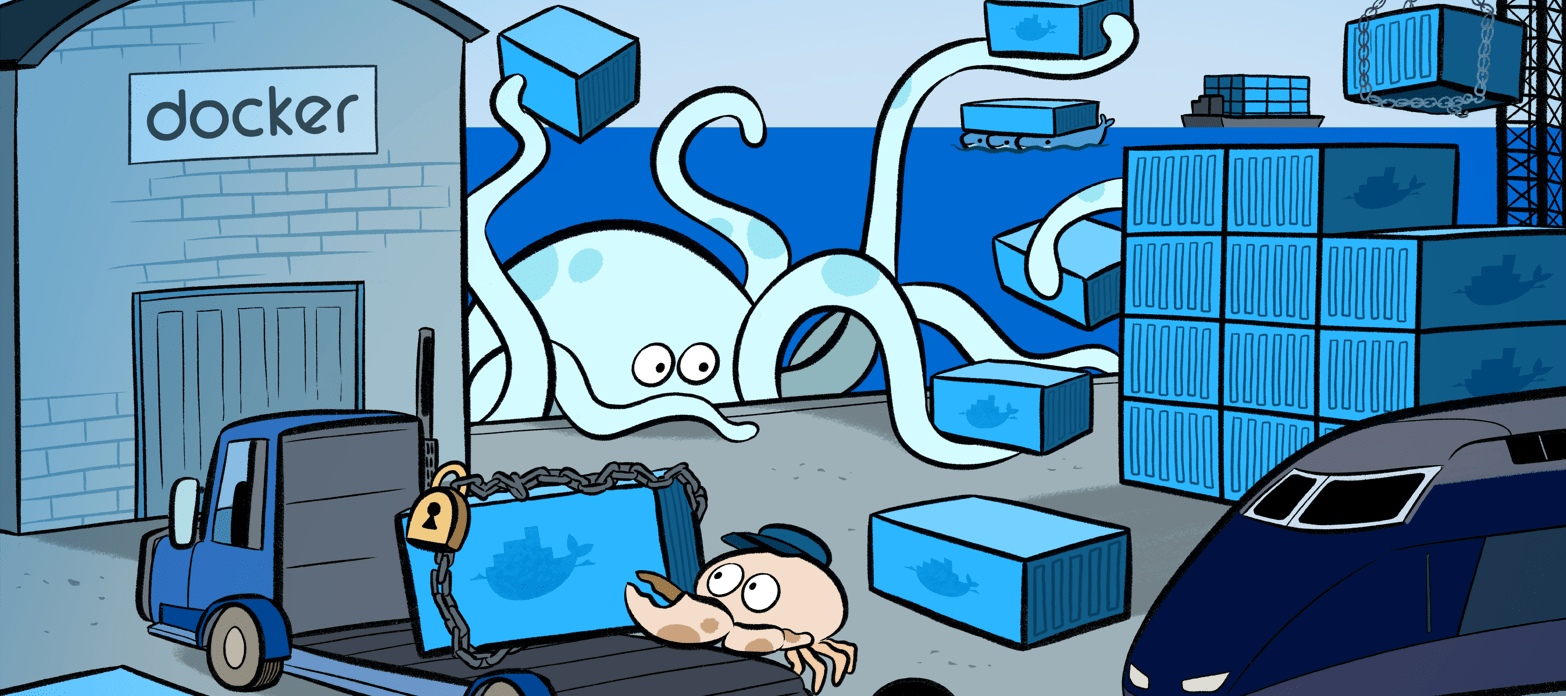
\includegraphics[width=1\textwidth]{docker.png}
\caption{https://www.docker.com}
\end{figure}

\textsf{간혹 주변에서 본격 웹 개발자가 되고 싶다}거나, 아니면 어떤 필요에 따라 웹 개발이라는 분야에 도전해 보려는 분들이 계신데, 마땅히 추천해 드릴 자료나 가이드가 너무 부족하다는 생각이 들었습니다. 그도 그럴 것이, 아직 웹 개발이라는 분야가 빠르게 성장하고 있고, 어제는 촉망받던 기술이 오늘의 레거시가 되버리는 상황이 반복되고 있어서, 정작 전업 개발자들조차 따라가고 배우기 벅찬 상황입니다. 뭐 하나 배워 놓으면 금세 쓰레기 지식이 되고 마는 거죠. 게다가 뭐 하나의 한 분야의 같은 일을 하는 데도 다양한 기술과 방법이 숱하게 쏟아지면서 서로가 좋은 방법이라며 싸움에 가까운 토론을 벌이고 있어서 혼란스럽습니다.

이런 상황에, 누군가 새로이 웹 개발에 도전해서 무언가 간단하게나마 만들고 싶다는 생각이 있다 하더라도, 무언가를 공부하고 있으면, 다른 누군가가 나타나서, 그게 아니라 이 방법이나 이 기술을 써야 한다며 훈수를 두는데, 잘 모르는 입장에서는 팔랑귀가 펄럭여서 새로 처음부터 시작하게 되기도 합니다.

맞습니다. 더 새로운 기술과 더 나은 도구들이 분명히 있습니다. 그런데, 개발자마다 성향과 상황과 또 그들의 과거 경험에 따른 선호도가 너무도 다르고 다양해서, 잘 정리된 가이드가 나오기는 힘들어 보입니다. 지금도 없었고, 앞으로도 없을 것입니다. 이 글 역시 그런 충분한 가이드일 수는 없습니다.

상황이 이러니, 이런 방법으로 도전해 보면 어떨까요? 우선 무언가 직접 만들어서 개발한 웹서비스를 온라인에 공개해 보는 겁니다. 아무도 안 쓰더라도 상관없습니다. 나 혼자 들어가 보고, 친구들에게 링크를 보내줍시다. 들어와 보고 ``이게 뭐냐?''라고 의아해하며 그냥 나가더라도 상관없습니다. 한번 만들어나 봅시다. 우아하고 최신의 기술이 아니어도 괜찮습니다. 일단 무언가 보이게 해 봅시다.


\section{목표}
이 글의 목표는 공부해야 할 주제와 키워드를 제시하는 것입니다. 그 상세 내용은 직접 찾아보며 하셔야겠지만, 전체 적인 계획과 꾸준한 노력을 투자할 기준점을 하나 세워드리는 것이 목표입니다. 취직이나 훌륭한 개발자가 되는 것이 목표도 아닙니다. 단지 내가 공부해서 웹서비스 하나 만들어 보는 것이 목표입니다. 안 그래도 어려운 개발, 생소한 개발, 목표를 간단하게 잡아 봅시다. 거창한 대규모의 웹서비스 아닙니다. 끽해야 백 명 쓸까 말까 한 서비스, 간단한 서비스입니다.

미리 말씀드리자면, 아무리 최대한 간단하고 얕게만 파고들더라도 긴 시간이 필요합니다. 일 투자 시간에 따라 다르겠지만, 수개월에서 수년이 넘게 걸릴 수도 있습니다. 이 글의 내용을 다 배우더라도 투자하는 노력에 비해 당장 눈에 보이는 결과가 보잘것없을 겁니다. 그럼에도 불구하고 시작해보겠다는 의지가 있으시다면 계속 읽어주시기 바랍니다.


\section{제공하는 가치}
개발 전체 과정에 있어 필요한 주제를 최소한 한 가지씩 꼽아드리겠습니다. 많아 봐야 두세 가지 중 하나를 택하면 되게끔 알려드리겠습니다. 접근하지 말아야 할 주제도 적어드리겠습니다. 시간을 낭비하는 함정에 빠질 일을 막아드리겠습니다. 당신이 뛰어야 할 젊은 말이라면, 양 눈 옆에 가리개를 가려드리겠습니다. 앞만 보고 뛰세요. 최단코스를 찾는라 고민하지 마세요. 우리의 목표는 갈팡질팡하지 않고 목적지를 향해 가는 겁니다, 조금 돌아가더라도요.

\section{제공하지 \dotemph{않는} 가치}
각 세세한 내용의 설명은 드리지 않습니다. 직접 해당 키워드로 찾아보시고 공부하셔야 합니다. 대부분의 내용은 이고잉님의 오픈튜토리얼스를 참고하시면 좋은 자료가 많을 것으로 생각합니다.

각 분야의 최고의 선택을 제시하지도 않습니다. 그저 되는 것 중에서, 제 개인이 선호하는 방법을 알려드립니다. 다른 개발자와의 의견은 얼마든지 다를 수 있습니다. 선택의 폭을 좁히는 것이 목표이지 최고 효율의 방법을 알려드리는 것이 목표는 아닙니다. 미리 귀뜀하자면, 이게 최선의 방법이다라고 주장하는 사람의 말을 듣지 마시라는 겁니다. 거짓말장이이거나 아직 무지한 사람일 가능성이 높습니다. 왜냐하면 이 바닥에서 최선의 방법을 제시하기는 꽤 어렵거든요.

\section{공부해야 할 주제}
정해진 카테고리는 아닙니다만, 대략 이렇게 나눠서 공략해 봅시다. 배우다 보면 한 주제에 대해서도 다양한 방법들이 즐비합니다.  언젠가 더 진지해진다면 더 깊게 다뤄야 하겠지만, 지금은 한눈팔지 말고 아주 얕게만 파기로 합니다. 누가 뭐라고 해도, 여기 정리한 선택만 하고, 나머지 선택은 외면해 버립시다. 이 주제들을 다 훑고 나면, 그 후에 누가 좋다고 한 기술을 더 알아보기로 합시다.

\begin{description}
\item[프론트엔드\textsubscript{front-end}] 이용자의 웹브라우저에서 직접적으로 보이는 부분을 다루는 기술
\item[백엔드\textsubscript{back-end}] 웹브라우저가 활용할 데이터를 기록하고 가져오는 등 뒷 단의 일을 처리하는 기술
\item[데이터베이스\textsubscript{database}] 백엔드가 다루는 데이터를 보관하고 검색
\item[네트워크\textsubscript{network}] 각 컴퓨터 사이의 데이터 통신
\item[에디터/툴/버전관리 시스템\textsubscript{tools}] 각 주제 개발 작업에 필요한 도구들 선택과 활용
\item[기초 자료 구조\textsubscript{data structure}] 데이터를 효과적으로 다루기 위한 기술
\item[리눅스/도커/AWS] 백엔드와 데이터베이스를 운영할 기술과 환경
\end{description}

아직 이 주제들이 무얼 의미하는지 몰라도 됩니다. 오늘 글에서는 이 주제들이 무얼 의미하고 어떤 걸 키워드로 전해드릴 지만 적어보겠습니다.

\section{프론트엔드}
흔히 \textsf{HTML, CSS, 자바스크립트\textsubscript{JavaScript}} 등의 단어를 들어보셨다면, 이 주제가 그 영역을 의미한다고 보시면 됩니다. 우리가 사용하는 웹브라우저가 이해하는 직접적인 기술들을 다루는 분야입니다. 인터넷 익스플로러, 사파리, 크롬 등의 웹브라우저는 인터넷에서 문서를 받아와서 화면에 보이는데, 이 보이는 문서의 내용들이 들어있는 모양새라고 보시면 어떨까 합니다.

다른 거 빼고, \textsf{HTML5, CSS3, JavaScript}를 보시면 됩니다. 서툴지만 쉽게 얘기하면, \textsf{HTML5}는 웹문서 본문을 적는 텍스트 포맷이고, \textsf{CSS3}는 그 문서의 스타일을 다루는 속성들이며, \textsf{자바스크립트}는 웹브라우저가 이해하고 실행할 수 있는 프로그래밍 언어입니다. \textsf{HTML5}와 \textsf{CSS3}는 평범히 적는 텍스트지만, \textsf{자바스크립트}는 좀 더 본격적인 프로그래밍을 해야 합니다.

프론트엔드 기술만 다뤄도 내 컴퓨터에 저장한 파일로 웹브라우저 화면에 무언가를 보이게는 할 수 있습니다.

보통 프론트엔드에서 무언가 주문(요청)을 하고, 그 주문을 멀리서 받은 서버가 응답을 주고, 그 응답 내용을 웹브라우저가 화면에 표시합니다. 프론트엔드가 먼저 요청을 해서 서비스를 받는 입장이고, 백엔드가 그 요청을 받아서 작업을 처리하고 응답을 주는 입장이라서 각각 클라이언트 측\textsubscript{Client-side}과 서버 측\textsubscript{Server-side}라고도 부릅니다. 식당에 가면 손님(클라이언트)이 주문을 하고 웨이터나 웨이트리스(서버)가 주문을 받아서 주방에 전달해 요리를 만들어 다시 손님에게 가져다 주는 상황과 비슷합니다.

이 기본 기술을 편하게 잘 다루기 위해, \textsf{React.js / AngularJS / Vue.js} 등의 다양한 추가 요소들이 있습니다. 우선은 거들떠보지도 말고, 오로지 \textsf{HTML5, CSS3, \dotemph{기본} JavaScript}만 봅니다. 자바스크립트를 다루는 데에도 그 앞에 \textsf{TypeScript}를 쓴다거나 더 효과적인 도구나 언어들이 있습니다만, 역시 우선은 빠져들지 많습니다. 그냥 날것의 자바스크립트만 봅니다.

특히 프론트엔드는 엎치락 뒤치락 새로운 기술들이 하루가 다르게 뒤엎는 분야입니다. 각별히 주의합니다.

아직 언급할 단계는 아니지만, 이 연재의 컨셉을 미리 밝히는 의미로 말씀드리면, 이런식이 될 것 같습니다.

프론트엔드에서 처리하는 내용이 더 방대해지고, 웹서비스의 수준이 올라가면서, 이용자의 기대치도 높아졌기 때문에, 위 기본 세 기술을 그대로 써서 원하는 결과물을 만들기는 어려움이 많습니다. 그래서 저 3가지 기술요소들을 더 유연하고 멋지고 편하게 다루기 위해 아래의 기술들이 쓰이는 상황입니다.

\begin{itemize}
\item 보통의 웹사이트 처럼 간단한 화면 요소들만 필요할 것 같다면 \href{https://vuejs.org}{Vue.js}를 공부해서 쓰세요.
\item 흔히 보는 웹사이트들 보다 우아하고 현란하게 바뀔 내용이 많은 경우에는 \href{https://facebook.github.io/react}{React.js}를 공부해서 쓰세요.
\item \href{https://angularjs.org}{AngularJS}는 시작도 하지 마세요. 덩치 큰 괴물입니다.
\end{itemize}

이런 컨셉이라서, 분명 \textsf{AngularJS}를 선호하시는 분들은 싫어하실 겁니다. 앞으로도 아마도 본인이 싫어하는 내용이 보이면, 이 시리즈 전체를 폄하하시거나 공격적인 의견을 피력하실 수도 있습니다. 이해합니다. 저라도 그렇습니다.

이 글의 목표는 \textsf{Vue.js / React.js / AngularJS} 같은 어려운 주제들을 고르는 노력조차 줄이는 데 있습니다. 그걸 고르고 평가하고 선택하는데도 굉장한 에너지가 듭니다. 혹자는 또 이렇게 얘기할 겁니다. 저 셋을 동일 선상에 놓는 것도 이상하다고, 정확한 의미를 규정하려 하며 태클을 걸 것입니다. 그분들의 말이 정확하고 맞습니다. 하지만 이 연재에서 저는 정확성을 포기하고 크로키로 전체 흐름만을 잡도록 하겠습니다.

\section{백엔드}

백엔드는 프론트엔드에 보일 자료들을 만들어 내는 영역입니다. 자바, 파이썬, 루비 등의 언어나 스프링, 장고, 루비 온 레일스 같은 프레임워크 이름을 들어보셨다면, 그게 바로 이 영역입니다.

백엔드에서는 프론트엔드에 보여줄 HTML 문서를 그때그때 생성해서 내려줍니다. 한번 작성하고 잘 바뀌지 않는 내용들은 평범한 파일의 형태로 디스크에 저장해뒀다가 전달해주고, 그때그때 변하는 새로운 자료들은 요청시 클라이언트마다 다르게 만들어서 내려주고는 합니다. 전자를 정적\textsubscript{static} 페이지라고 하고, 후자를 동적\textsubscript{dynamic} 페이지라고 합니다. 모든 고객이 같은 걸 보는 메뉴판 같은 것을 정적\textsubscript{static} 자원이라고 보면 되고, 고객마다 다른 응대를 해주는 웨이터/웨이트리스의 응대 기술이 동적\textsubscript{dynamic} 영역이라고 보시면 될 것 같습니다.

백엔드는 여러 고객의 요청을 한꺼번에 받아서 각각 제대로 처리해서 내려줘야 하는 동시성\textsubscript{concurrency} 처리 문제가 있어서 어려운 면이 있습니다. 요리 주문을 받은 주방에서는 요리사들이 다양한 재료를 한꺼번에 조리하면서 여러 요리가 각각 하나의 요리로 완성돼야 하는 상황과 비슷합니다. 요리사가 스테이크 요리를 하고 있는데, 스파게티 주문이 들어왔다고 해서 스테이크 요리에 토마토소스를 얹으면 안 되잖아요? 그렇다고 스테이크 요리가 끝날 때까지 기다렸다가 스파게티 요리를 시작하면 고객들은 이미 화를 내며 집에 갈 테고요. 그러니 여러 가스레인지에 여러 요리가 마구 동시에 조리돼야 하는데 이렇게 동시에 여러 작업을 하면서도 각각의 처리 단위가 서로 꼬이지 않게 완성되게 하는 일이 동시성 처리입니다. 동시성 처리를 잘 하면서, 성능까지 좋아야 많은 고객의 다룰 수 있기 때문에 다양하고 어려운 기술들이 많이 있습니다만, 우리의 목표는 대용량 서비스가 아닙니다. 간단한 서비스이므로, 동시성 처리를 문제없이 다루되, 빼어난 성능을 위한 기술들은 외면하도록 합시다. 동네 맛집을 운영할 거지 특급호텔 뷔페 주방을 운영할 게 아니거든요.

백엔드는 특히 성능 튜닝의 작업이 효과적으로 드러나는 분야라, 아주 사소한 영역까지 더 빠르게 개발하려는 노력이 깃드는 분야입니다만, 지금은 불필요한 잡기로 여기고 거들떠보지도 말도록 합니다.

백엔드는 특성상 프로그래밍 언어의 선택이 자유롭고 다양합니다. 앞서 언급한 대로 흔히 \textsf{Java, Python, Ruby} 등이 흔히 선택되고,  프론트엔드의 자바스크립트 언어를 백엔드에서 쓰는 \textsf{Node.js}도 있고, \textsf{Go}나 \textsf{Swift} 같은 언어도 있습니다. 제가 즐겁게 배우고 있는 \textsf{Clojure}도 쓸 수 있습니다만, 우선은 \textsf{Python}이나 \textsf{Ruby}중에서 고릅니다. 둘 다 가볍고 빠르게 더 많은 결과물을 만들어 낼 수 있습니다. 주변에서 \textsf{Java}를 권하는 사람들이 있을 텐데, 고맙다 말하고 무시하세요.

\textsf{Python}과 \textsf{Ruby} 프로그래밍 튜토리얼 사이트를 빠르게 훑어보시고, 조금이라도 더 끌리는 쪽으로 선택해서 백엔드 개발에 활용하시면 됩니다. 저 개인적으로는 \textsf{파이썬}이나 \textsf{루비}나 비슷해 보이고, 둘 중에는 \textsf{루비}를 선호합니다만, 적어도 국내 상황에서는 \textsf{루비}는 다소 식어있고, \textsf{파이썬}은 꽤나 흥하고 있습니다. \textsf{파이썬}의 경우 매년 열리는 컨퍼런스의 규모나 참석자 수를 보더라도 흥하고 있는 것을 알 수 있습니다. 다만, 웹 개발에는 \textsf{루비 온 레일스}라는 극강의 프레임워크가 \textsf{루비} 쪽에 있기 때문에, 딱 둘 중에 뭐다 우세를 정하기 어렵습니다. 국내 커뮤니티 규모의 측면에서는 \textsf{파이썬}, 웹개발의 편리함 측면에서는 \textsf{루비}를 선택하면 되겠습니다. \textsf{파이썬}도 \textsf{장고} 같은 프레임워크가 잘 돼있기 때문에 아주 큰 차이는 아닐 겁니다.

다만, \textsf{Java}는 무시하도록 합니다. 우리가 짓고자 하는 것은 2층 목조 주택인데, 대형 아파트 단지를 지을 언어를 선택할 이유는 없습니다. 그리고, 프론트엔드 개발부터 시작하신 분들은 자바스크립트 언어를 써서 백엔드 개발을 하는 \textsf{Node.js}를 선택하기도 합니다. 나쁘지 않습니다만 일단 제외합니다. 쉽게 접근할 수 있는 \textsf{PHP}를 권하는 사람도 있을 겁니다. 고맙다 말하고 무시하세요.

\begin{itemize}
\item \emph{Do} -  루비나 파이썬 중에 고르세요.
\item \emph{Don't} - 자바나 PHP는 거들떠보지도 마세요.
\end{itemize}

\subsection{흘러가는 기술들}

이 글의 방향성을 밝히고자, 조금 미리 \textsf{React나 Vue.js} 같은 주제를 말씀드렸습니다만, 다시 강조하자면, 그런 주제를 시작하기에 앞서서 \textsf{HTML5, CSS3, Javascript} 기초를 먼저 닦아두는 편이 좋습니다. 흔히 우리는 무언가 공부해야 하는 주제가 쌓여있을 때, 조급한 마음에 기초를 건너뛰고 지금 당장 쓰이는 기술에 먼저 접근하려는 유혹에 빠지는데, 그래 봤자 다시 기초로 돌아와야 해서 오히려 더 느리게 나아가게 되기도 합니다. 유행하는 기술을 빨리 공부하고 싶은 조급한 마음은 잠시 가라앉히고, 기초부터 닦는 게 실질적 도움이 더 크기도 해요. 그리고, 어차피 \textsf{React나 Vue.js} 같은 것들은 2~3년이 지나면 또 언제 핫했냐는 듯 금세 유행이 가고 더 새로운 기술로 그 관심이 옮겨갑니다. 빠르게 변하는 분야는, 어제의 핫한 기술이 오늘의 폐품이 되는 주기가 굉장히 짧습니다.

그래서 기초를 잘 쌓으면서, 그 위에 유행하는 기술은 잘 익혀서 유통기한 내에 잘 써먹고 잊으면 됩니다. 핫한 기술들은 지식을 축적하는 게 아니라 소비하는 일이라고 보면 좋습니다. 잘 씹어 먹고 잘 소화해서 그 날의 에너지원으로 삼으면 됩니다. 굳이 그 지식들을 뼛속 깊이 쌓아둘 필요는 없어요. 너무 오래 쌓아두면 오히려 독소가 됩니다. 반면, 기초가 되는 기술들은 뼈로 만들기까지 시간이 좀 들고, 당장은 쓸모없어 보이기도 합니다만, 일단 뼈가 되고 나면 그 위에 지방을 쌓든 근육을 키우든, 중요한 버팀목이 되어줍니다. 뼈와 지방은, 어느 한쪽이 중요하고 다른 쪽이 덜 중요한 것이 아니라, 성격과 활용이 다른 것뿐이고 둘 다 중요하고 필요합니다. 다만 보통 초심자들이 겉에 잘 드러나는 지방과 근육에 쉽게 현혹되기 때문에, 이 연재에서는 균형을 맞추고자 뼈를 만드는 쪽을 좀 더 강조하는 입장을 취하도록 하겠습니다.

다시 말해 \textsf{React나 Vue.js}는 요새의 \emph{칼로리원이나 근육으로 삼으면} 되고, \textsf{HTML5, CSS3, Javascript}로는 \emph{탄탄한 뼈를 만들면} 됩니다. 뼈가 없으면 애써 근육을 만들어봐야 지지대가 없어서 힘을 쓸 수 없겠죠? 한편, 우리 몸의 뼈도 보통 6개월이 지나면 완전히 새로운 세포로 교체된다고 하더군요. 기초 기술이라고 해서 영원한 것은 아니고, 단지 지방이나 근육보다 조금 더 오래가는 것뿐이에요.

자, 그럼 이제 모호한 얘기는 이쯤에서 줄이고, 이어서 이번 편에는 ``데이터베이스''와 ``네트워크''에 대해 어디서부터 공부하면 좋을지 정리해볼게요.

\section[database]{데이터베이스\textsubscript{database}}

드디어 우리 웹서비스의 데이터를 저장할 방법을 알아볼 때입니다. 보통 프론트엔드와 백엔드는 오가는 데이터를 처리하면서 일시적인 부분만을 잠깐씩 기억하면서 활용하며, 실제로 오래 보관할 내용은 데이터베이스에 기록합니다.

데이터베이스의 사전적 의미는 ``잘 정돈한 데어터의 모음''입니다. 우리가 필요한 데이터를 잘 기록하면서, 필요한 때에 찾아보기 좋게 잘 정돈해 놓는 거지요. 흔히 약자로 DB라고 부르는데, 데이터 모음을 포함해서, 그 데이터 모음을 관리하는 시스템이나 소프트웨어를 뭉뚱그려 부르기도 합니다. (정확하게 말하자면, 후자는 DBMS라고 구분해서 말해야 하는데 그러지 않아도 널리 이해하는 분위기인 것 같습니다.)

DB도 종류가 여럿인데, 가장 널리 쓰이는 것은 RDB라고 관계형(Relational) 데이터베이스입니다.  MySQL, PostgreSQL, Oracle 등이 RDB이지요. 대부분 RDB를 쓰기에 DB라고만 해도 RDB를 뜻하기도 합니다.

DB에 컬럼, 레코드, 테이블의 구조를 갖춰 데이터를 기록하는데, 이는 우리가 흔히 쓰는 스프레드시트 프로그램의 구조와 비슷합니다. 엑셀이나 구글시트의 시트가 DB의 테이블이고, 각 시트의 행이 레코드이며, 열이 컬럼입니다. 엑셀로 가계부를 정리할 때, 날짜/내역/금액/비고 등의 열을 두고, 각각의 행에 입출금 내역을 적어 놓는 것과 같습니다.

\begin{tabular}{|c|c|c|}
  \hline
  가계부(시트) & => & 테이블  \\
  날짝/내역/금액/비고(열) & => & 컬럼 \\
  일출금 내역(행) & => & 레코드 \\
  \hline
\end{tabular}

영수증을 어딘가에 잘 쌓아두기만 해도 될 텐데, 왜 굳이 엑셀에 힘들게 적어 놓나요? 기초 자료를 바탕으로 잔액이나 총 지출/수입 등을 자동으로 계산할 수 있고, 특정 날짜의 항목을 찾거나, 내역의 텍스트나 금액을 기준으로 검색해서 찾아보기 쉽기 때문 아닌가요? 기록으로 보관하려는 의도도 있고, 계산과 검색이 편한 구조로 남겨두는 목적도 있습니다.

엑셀 등에 담는 시트가 테이블인 셈인데, 관계형 데이터베이스는 그 안의 여러 테이블 사이에 관계를 다루는 연산들이 있습니다. 한 테이블만을 대상으로 해서 계산하거나 검색하는 범위를 넘어서, 두 테이블 이상을 합쳐서 무언가 계산하거나 검색하는 경우도 많습니다.

DB에 연산을 요청하는 내용을 쿼리\textsubscript{query}라고 부릅니다. 우리말로 `질의'라고 번역하거나 그냥 쿼리라고 부릅니다. 이 쿼리는 꽤 유연하고 강력한 기능들이 많이 필요하기에, 하나의 언어로 되어있습니다. 이 언어의 표준 격으로  SQL\textsubscript{Structuered Query Language}, 구조화된 질의 언어)이라는 것이 있고, 각 DB 제품마다 조금씩 다른 방언\textsubscript{dialect}을 씁니다. 서울말을 바탕으로 한 표준어가 있고, 각 지방에서 쓰이는 방언들이 조금씩 다르지만 대개는 의사소통이 되는 것 상황과 비슷합니다. MySQL에서 쓰는 쿼리와, PostgreSQL에서 쓰는 쿼리가 거의 비슷하면서도 세세한 부분이 조금씩 다릅니다.

휴, 여기까지만 해도, 앱 개발을 위해 자바스크립트, (루비 or 파이썬), SQL까지 세 개의 복잡해 보이는 언어를 배워야 하게 되었네요. HTML도 사실상 마크업 \dotemph{언어}이기 때문에 그런 것까지 언어라고 말하면 금세 더 배워야 할 언어의 수가 늘어납니다. 하지만, 언어라고 해서 너무 겁먹을 필요는 없습니다. 영어나 중국어를 배우는 것처럼 어려운 일은 아닙니다. 문서도 잘 돼있고, 보통 좋은 언어들은 그 표현 자체가 단순하며, 무엇보다 쓰는 순간마다 도와주는 도구가 아주 잘 돼 있어서, 대충 얘기해도 철석같이 잘 알아들을 수 있는 표현으로 바꿔주며, 조금이라도 틀린 표현이 나오면 자동으로 알려줍니다. 내가 콩글리시로 대충 얘기해도 늘 따라다니는 미국인이 그 자리에서 정확한 표현으로 통역해주는 상황이랄까요? 다만, 너무 어긋나면 통역이 불가능하겠지만요.

아무튼, 이쯤에서 DB도 제품을 골라야 하겠습니다. 지금 상황에서는 MySQL이 가장 널리 쓰이는 것 같습니다. 책도 많이 나와있고요. 다만 저 개인적으로는 MySQL이 오라클에 인수됐기 때문에 능동적으로 발전해 나가야 할 이유가 줄어들었다고 생각합니다. 아마 그 흐름을 MariaDB가 이어받는게 아닌가 합니다만, 그냥 전 속 편하게 PostgreSQL을 쓰자는 입장이기에 잘 모르겠습니다. 안전한 선택을 하시려면 MySQL, 그 보다는 마이너하지만 제대로 된 선택을 하시려면 PostgreSQL을 택하시면 되겠습니다. 그렇다고 MySQL이 제대로 된 것이 아니라는 뜻은 아닙니다. 아 참 이거 조심스럽네요. 매번 말씀드리듯, 적지 않은 기술적 선택에 개인 취향이 많이 작용합니다. 정리하자면, MySQL이나 PostgreSQL 중에 고르면 됩니다. 이 역시 주변에서 Oracle이나 Microsoft SQL Server 등을 권하기도 할 겁니다. 고맙다 말하고 무시합니다. 마침 서울에 출장 온 김에 대형 서점에 들러서 둘러 보았더니, 역시나 오라클과 SQL Server 책이 많더군요. 아무래도 기업들이 많이 쓰는 제품이라 그런 것 같습니다. 우리는 기존 기업에 취직해서 DBA가 될 게 아니라, 내가 원하는 작은 웹서비스를 만들 것이므로 깔끔히 외면하도록 합니다. 그래도 MariaDB나 MySQL 책은 더러 있었는데, 아쉽게도 PostgreSQL책은 레퍼런스 사이트를 번역한 책 한 권 밖에 찾지 못했습니다. 그래서 PostgreSQL로 선택하신다면, SQL 기본 서적을 보면서 공식 웹사이트 매뉴얼을 참고하시는 방법이 좋을 것 같습니다.

한편, DB는 데이터를 보관한다는 측면에서 워낙 중요하고, 또 오랜 기간 중요하게 기능하며 발전해 왔기에, 이용하는 입장에서도 어렵지만, 그걸 관리하고 운영하는 입장은 훨씬 더 어려운 면이 있습니다. 데이터를 잘 남겨두고, 주기적으로 백업(별도 보관)하고 혹시라도 장애가 나면 복구해야 하며, 때로는 데이터를 다른 곳으로 옮겨야 하며, 새로 구축해야 할 때도 있습니다.  관리\textsubscript{Administration}의 측면만 봐도 큰 일이고 전문적이어서 그 직종이 따로 있고, 큰 회사들은 전담 팀과 부서가 따로 있는 경우가 많습니다. 그러나 역시 겁먹을 필요는 없습니다. 2층 집을 짓는 우리에게는 별도 인력을 확보할 여력이 없기도 하고, 다행히도, 앞으로 사용할 AWS 같은 환경에서는 그 관리의 행위와 역할이 클라우드 쪽으로 대폭 옮겨 가서, 개발자가 직접 해야 할 일이 훨씬 줄었습니다. 백업이나 복구 같은 일만 해도 꽤 어렵고 힘든 일인데, 요새는 AWS 콘솔에서 클릭 몇 번 하면 알아서 잘 해주지요. 아직 설명하지 않은 시스템 운영 측면에서도, 이 시대의 인프라 시스템이 너무 잘 돼 있어서, 사실 그 어느 때보다도 한 개인이 완전한 서비스를 만들어 내기 쉬운 환경이 됐습니다. 앞으로 더 쉬워지겠지요.

다시 데이터베이스의 이용 측면으로 돌아와서, 웹 개발자 입장에서는 우리가 고른 루비나 파이썬 백엔드 프로그램에서 데이터베이스에 접근해서 새 데이터를 기록하거나, 이미 기록한 데이터를 잘 조회해서 보여주는 일을 합니다. 그때 우리가 만드는 백엔드 소프트웨어(웹서비스)가 DB와 통신하기 위해 사용하는 언어가 SQL입니다. 백엔드가 직접 SQL을 거의 그대로 쓰는 경우는 요새는 별로 없고, 그 사이에 조금 더 편리한 계층이 있습니다. 루비온레일스의 경우에는 액티브레코드\textsubscript{ActiveRecord}라는 라이브러리가 그 일을 합니다. DB서버가 다루는 집합(set) 구조의 레코드와 컬럼을 객채지향 프로그램에서 다루기 좋은 형태로 변환하는 일을 하지요. 이 형태가 아직 통일된 것은 아니라, 각 언어별로 조금씩 다른 구조를 취하기도 합니다. 예를 들어 자바에서는 JPA라는 표준이 있어서 그런 일을 담당합니다. 루비온레일스의 액티브레코드 같은 경우는, 적어도 제가 써 본 것들 중에는 가장 우아하고 강력한 기능을 자랑했습니다. 아무래도 이질적인 무언가를 매개하는 일을 할 때는 보다 유연한 언어가 유리한 것 같습니다.

액티브레코드처럼 훌륭한 지원 도구가 있는 경우에는 SQL을 아주 기본적으로만 알아도 됩니다. 복잡한 구문들을 액티브레코드가 대신 처리해주니까 말이죠. 하지만, 그렇다고 SQL을 몰라도 된다는 뜻은 아닙니다. 복잡하고 번거로운 작업을 아주 편리하게 대신해주는 겁니다.

그래서 DB를 하나 골라서, SQL의 기초를 공부해가며 테이블과 관계를 다루는 법을 익히면서, 우리가 택한 언어에서 널리 쓰이는 DB 접근 레이어를 써서 유연하게 데이터를 다룰 수 있게끔 공부하면 되겠습니다.

\begin{itemize}
\item \emph{DO} - MySQL or PostgreSQL
\item \emph{DON'T} - Oracle nor SQL Server
\end{itemize}

완전히 다른 얘기로, 데이터베이스라는 것이 결국, 우리가 만드는 웹서비스에 잘 정리하고 나중에 찾아볼 데이터를 잘 다룰 수 있으면 되는 겁니다. 그 형태가 꼭 관계형 DB일 필요는 없지요. 만약 그냥 디스크에 파일로 저장하거나 엘라스틱 서치 같은 검색 엔진에 부어 넣고도 내가 원하는 기능을 만들 수 있다면 그렇게 쓰면 됩니다. 그래서 RDB 말고도 MongoDB나 AWS의 DynamoDB를 비롯해서 다양한 형태의 데이터베이스가 널리 쓰이고 있습니다. 어쩌면 사람들이 너무 RDB에 치우쳐 있기에, 경우에 따라 다른 방식의 접근이 더 좋은 경우도 있다는 것을 잊게 되기도 하는 것 같습니다. 그리고 RDB를 쓴다고 해서 반드시 100\% 모든 데이터를 RDB에 담아야 하는 것도 아닙니다. 대부분은 RDB에 담고, 경우에 따라서 다른 형태로 저장해도 되지요. 그러니 RDB를 공부한다고 해서, 세상의 데이터베이스가 RDB가 전부다라는 생각으로 굳어지지는 말아야 하겠습니다. 분명, RDB는 오랜 기간 발전하면서 매우 성숙한 제품과 기술들이 함께 진보했기 때문에 가장 안전한 선택입니다만 말이죠.

한 가지 더, 한 귀로 흘려들으실 여담으로, 제가 만약 RDB 외에 선택 다른(?) DB를 쓴다면 Datomic이라는 제품을 쓰겠습니다. 아직 널리 알려지지 않았고, 상용 제품이기에 접근성이 떨어집니다만, 불변\textsubscript{immutable} 데이터베이스라는 점이 아주 매력적으로 보입니다. 아직은 좀 기다려 봐야죠. 발상과 접근이 너무 좋아서, 곧 비슷한 접근 방식을 취하는 오픈소스 제품이 나와서 함께 발전하지 않을까 생각하고 있습니다. 그리고 조금 더 용기가 난다면, 돈을 내고라도 써 볼 만한 제품이라고 눈독 들이고 있습니다. 유료라고 해서, 오라클 같은 대기업용 제품처럼 막대한 비용이 필요한 건 아니니까요. 아니면, AWS위에서 과금제로 쓰는 만큼 돈을 내는 Datomic이 출시될 수도 있으니, 그걸 써도 괜찮지 않을까 합니다.

괜한 딴 얘기를 했네요. 우선 RDB 하나 골라서 공부하며 씁시다! RDB의 단점으로 지적되는 부분들이, 적어도 우리가 목표로 하는 동네 웹서비스 영역에서는 문제점으로 드러날 일은 없다고 생각해요. 나중에 AWS를 언급하면서 RDS 서비스를 말씀 드릴 텐데, MySQL, PostgreSQL 다 편하게 쓸 수 있으니, 고르시기만 하면 됩니다. \emph{거 참 좋은 세상!}

\begin{quote}
  \emph{요약} - MySQL이나 PostgreSQL을 고르고, SQL을 공부해 가며, 내가 택한 언어의 DB 접근 라이브러리를 써서 연습한다.
\end{quote}

\section{네트워크}
네트워크야 익숙하시죠? 우리 어디 가서 WiFi 안되면 공황상태에 빠지잖아요? 너무 익숙해서 모른다고 말하기 민망할 지경이죠. 우리 장비들이 서로 통신하는 망을 네트워크라고 합니다. 오래전에는 다른 네트워크 방식이 많았지만, (지금도 은행같은 금융권이야 다른 망을 많이 쓰겠지만) 요새야 네트워크라고 하면 인터넷을 의미하는 거죠. 간단하게만 얘기하자면, 우리가 쓰는 컴퓨터와 저 멀리 있는 백엔드 서버와 통신하는 연결선이라고 생각하면 어떨까 합니다.

어떤 장비가 네트워크에 연결되면, 고유의 주소를 할당받습니다. IP라고 줄여 부르는 이 주소가 인터넷에서의 주소입니다.  Internet Protocol 주소의 약자인데, 인터넷에서 쓰는 주소라고 생각하시면 되겠습니다. 모든 장비에 이 IP주소가 있어야 서로 통신이 됩니다. 내가 편지를 어디론가 보내려면, 받는 사람 주소가 있어야 하는 것처럼 당연한 일입니다. 생긴 모습은,

\begin{quote}
104.74.171.196
\end{quote}

이렇게 네 뭉치 숫자가 마침표로 이어진 모양으로 생겼습니다. 각 숫자가 1바이트라서 최대 255까지 표현합니다. 숫자상으로는 `0.0.0.0`부터 `255.255.255.255`까지 표현할 수 있습니다만, 중간중간 영역이 특별한 용도로 제외되기 때문에 모든 숫자를 다 쓰는 것은 아닙니다. 이렇게 4바이트로 인터넷 주소를 쓰는 것을 IPv4(Internet Protocol version 4) 주소라고 합니다. 특별한 목적으로 제외된 영역을 빼고 단순하게 계산해도 4바이트로는 $2^{32}$인 42억 개 정도를 쓸 수 없습니다. 이 주소를 IANA라는 단체에서 영역으로 떼어서 전세계 인터넷 서비스 제공업체에 할당해 주는데, 2011년 3월에 동이 났다고 하는군요. 실제로 전세계에서 42억 개 정도를 다 쓰는 것은 아니겠지만, 과잉 할당된 곳도 있을 테고, 또 워낙 세상에 장비들이 많으니 그럴 만도 합니다.

그래서 IPv6(Internet Protocol version 6) 주소를 쓰게 됩니다. 16바이트로 인터넷 세상의 주소를 표현하는 거지요. 16바이트로 표현하면 $2^{128}$ 개의 주소를 표현할 수 있으므로, 적어도 우리가 살아있는 동안에 부족할 일은 없어 보입니다.

\begin{figure}
\centering
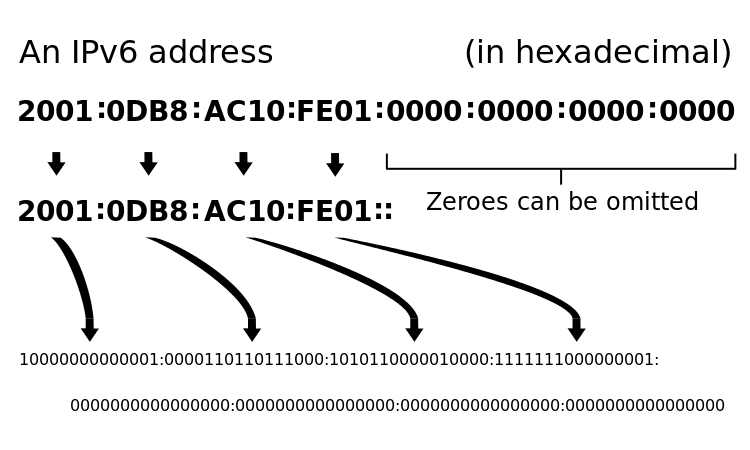
\includegraphics[width=\textwidth]{ipv6_address.png}
\caption{IPv6 주소 <\url{https://en.wikipedia.org/wiki/IPv6}>}
\end{figure}

이렇게 생겼다는데, 거 참 생소하네요.

요새야 거의 모든 장비와 서비스가 IPv4와 IPv6를 함께 지원하지만, 적어도 국내 환경에서는 그다지 호응이 없어 보입니다. 정확한 이유야 모르겠지만, 아마도 우리나라에 할당된 IPv4 주소 영역이 매우 넉넉하기 때문이 아닐까요? 부족하지 않으니 아쉬울 것이 없어서 우물을 팔 필요가 없는 거지요. 그래서 아직은 IPv4 만 알아도 되겠습니다만, 좀 익숙해지고 나서 IPv6도 신경 쓰면 좋겠지요.

IPv4건 IPv6건, 이 주소로 원하는 목적지에 요청을 보내야 하는데, 보시다시피 이 주소는 우리가 일일이 외우기는 어렵습니다. 네이버나 구글에 접속해서 검색을 해봐야 하는데, 저런 숫자로 접근해서 봐야 한다면 참 골치 아픈 일이 아니겠습니까?

그래서 전화번호부 역할을 해주는 서비스가 있습니다. 114 전화해서 ``네이버'' 얘기하면 ``네이버'' 전화번호를 알려주는 것처럼요. 그럼 우리는 여러 서비스의 전화번호를 외우지 않아도 됩니다. ``114''라는 전화번호 하나만 외우고 있으면 되지요. 그런 전화번호부 역할을 해주는 것이 DNS입니다. 도메인 이름 시스템\textsubscript{Domain Name System}이라고, 우리가 읽을 수 있는 문자로 표현합니다.

\begin{quote}
www.naver.com
\end{quote}

이렇게요. 저 이름이 사실은 `104.74.171.196'를 대신하는 주소명인 겁니다. 저 주소명을 IP주소로 알아내는 작업을 DNS 조회\textsubscript{look up}라고 합니다. 114에 전화 걸어서 상표명 묻는 행위인 거죠. 난 114를 입력한 적이 없는데 어떻게 그런 일을 하냐고요? 우리 장비가 인터넷에 연결되면, 우리 장비에 임시 IP주소를 할당해 주면서 DNS 서버 주소도 함께 줍니다. 그 114 역할을 하는 IP주소를 우리 컴퓨터나 스마트폰의 장비가 잘 기억하고, 그때그때 물어봐가며 IP 주소를 가져와서 원하는 목적지에 연결해 주는 작업을 합니다.

IP주소도 유한한 자원입니다만, 저 도메인명도 희소한 유한 자원이기에, 돈을 주고 삽니다. 1년에 돈 만원 정도 내면 해당 이름을 내가 원하는 IP주소에 연결하는 일을 해둘 수 있습니다. 자기 블로그 자기 도메인 명으로 운영하는 사람들 있죠? 그 도메인을 도메인 등록 서비스 업체에서 산 거에요. 우리도 돈 만원쯤 내서 사면 우리 백엔드 서버들에 할당된 IP주소로 쉽게 접근할 수 있도록 전화번호부\textsubscript{DNS}에 등재해 둘 수 있습니다.

DNS를 거쳐서 알아내든, 직접 외우고 있었든 이제 IP주소를 알았습니다. 그다음 포트에 대해서 알아볼게요. IP주소는 보통 한 장비를 의미하고, 한 장비 내에서도 포트\textsubscript{port}라는 것이 여러 개 있습니다. 포트는 2바이트로 0~65535 사이의 숫자를 씁니다.  0번과 49152번 이후의 숫자를 특별한 용도로 제외하고 그 사이의 숫자로 약 5만 개의 포트를 쓸 수 있습니다.

포트는, 반드시 그런 것은 아닙니다만, 각 통신 목적에 맞는 포트 번호 관례가 있습니다. 예를 들어 우리 웹브라우저로 접근하는 웹서비스의 경우 80번 포트를 써요. 암호화된 통신의 경우는 443번 포트를 쓰고요. 웹서비스 통신에 오고 가는 데이터 규약을 HTTP라고 부르는데, 이걸 암호화하지 않고 주고 받는 경우는 80번 포트로 접근하고, 암호화해서 주고 받는 경우에는 443번 포트에 접근합니다.

즉, 브라우저에서 아래처럼 치는 것은

\begin{quote}
http://www.naver.com/
\end{quote}

사실상

\begin{quote}
http://www.naver.com:80/
\end{quote}

과 동일합니다. 저런 주소 전체를 URL이라고 부르는데, 앞에 `http'가 프로토콜이고 `www.naver.com'이 도메인 명이며 `80'이 포트번호입니다. 암호화한 데이터를 주고받는 `https'의 경우는,

\begin{quote}
\quote{https://www.naver.com/}
\end{quote}

으로 접근하고, 이는 사실상

\begin{quote}
\quote{https://www.naver.com:443/}
\end{quote}

으로 접근한 것과 같습니다. 이 글을 쓰는 현재 http로 네이버에 접근하면, 자동으로 암호화된 https로 다시 연결하게 처리해주네요. 무조건 암호화된 통신을 하겠다는 얘기입니다.

우리가 웹서비스를 만들면 우선 80 포트 기준으로 백엔드 서비스를 띄워놓고 개발하다가, 나중에 도메인도 사고, 친구들에게 공개하기 전에는 폼나게 443번 포트에 암호화된 웹서비스를 올려두도록 합시다. 여기에는 TLS 인증서를 발급받아서 올려놓아야 하는데, 요새는 무료로 제공하는 서비스도 있기에 아주 어려운 일은 아닙니다. 혹시 연재가 길어진다면 그 부분도 적도록 할게요.

네트워크도, 조금 살펴보니 의외로 재밌지 않나요? 더 관심이 가신다면 네트워크 관련 서적을 더 살펴보시면 제 어설픈 설명보다 훨씬 잘 정리된 내용을 보시기 좋을 거예요.

그다음으로, 네트워크 기초를 보고 나면, 웹브라우저와 우리가 만들 백엔드 서버가 HTML, CSS, Javascript 파일 등을 주고받을 때 쓰는 프로토콜인 HTTP에 대해서도 살펴보도록 합시다. HTTP는 현재는 버전 1.1이 널리 쓰이고 있고, 2.0도 거의 모든 웹브라우저가 지원하며, 2017년 5월 기준, 상위 1천만 개의 웹사이트 중 13.7\%가 지원하고 있다고 나와있으나, 체감상 아직 널리 쓰이는 것 같지는 않습니다. 이 점도, 아쉬운 사람이 우물을 파야 하는데, 구글이나 네이버 같은 대형 서비스 제공업체에서나 엄청난 망 비용을 절약하고 싶어서 아쉬운 거지, 소규모 서비스 제공자 입장에서야 그다지 아쉬운 상황이 아니라서 말이죠. 그래도 언젠가는 2.0이 널리 쓰이겠지요. 아마도 IPv6가 안착할 때쯤? ㅎㅎ

이상 네트워크는, 제가 쉽게 설명하기에는 좀 무리가 있는 카테고리였음을 인정합니다. 솔직히, 뭐라고 요약해야 할지도 잘 모르겠네요.

\begin{verse}
요약: 인터넷 네트워크 기초 서적을 한 권 살펴보고, HTTP/1.1 프로토콜의 기초를 파악한다.
\end{verse}

\section{텍스트 에디터}
\section{통합 개발 환경}
\section{버전 관리 시스템}
\section{기초 자료 구조}
\end{document}
